% Please do not change the document class
\documentclass{scrartcl}

% Please do not change these packages
\usepackage[hidelinks]{hyperref}
\usepackage[none]{hyphenat}
\usepackage{setspace}
\doublespace




% You may add additional packages here
\usepackage{amsmath}
\usepackage{cite}
\setlength{\parindent}{4em}
\usepackage{graphicx}

% Please include a clear, concise, and descriptive title
\title{Do the benefits from early and frequent user research outweigh the potential cost on the return on investment for games?
}

% Please do not change the subtitle
\subtitle{COMP150 - Agile Development Practice}

% Please put your student number in the author field
\author{1703170}

\begin{document}

\maketitle

\textit{One of the major factors that contribute to a games success at launch is the ability to recognise and fix problems with the game before release. But does too much user research and playtesting negatively impact development?  This paper outlines how user research is implemented using Agile development methods and how these methods affect development time and costs compared with other less rigorous methods in the games industry.  }

\section{Introduction}

User research is a vital part of a games development and allows a developer to gather important data about the game like metrics (see fig.1). But how much user research is appropriate for your game? Production teams that take an Agile approach \cite{fowler2001agile:1} to game development often implement user research early on in the process and yield positive results when implemented well, while others that prefer plan-based approaches to game development do the majority of their playtesting and user research towards the end of the development process. Often these can lead to issues at launch. The purpose of this paper is to discuss the positives and negatives of an Agile and iterative approach to game design with reference specifically to that topic of user research. The paper will compare and contrast these findings to the methodology they used in development \cite{politowski2016old:2}.

\begin{center}
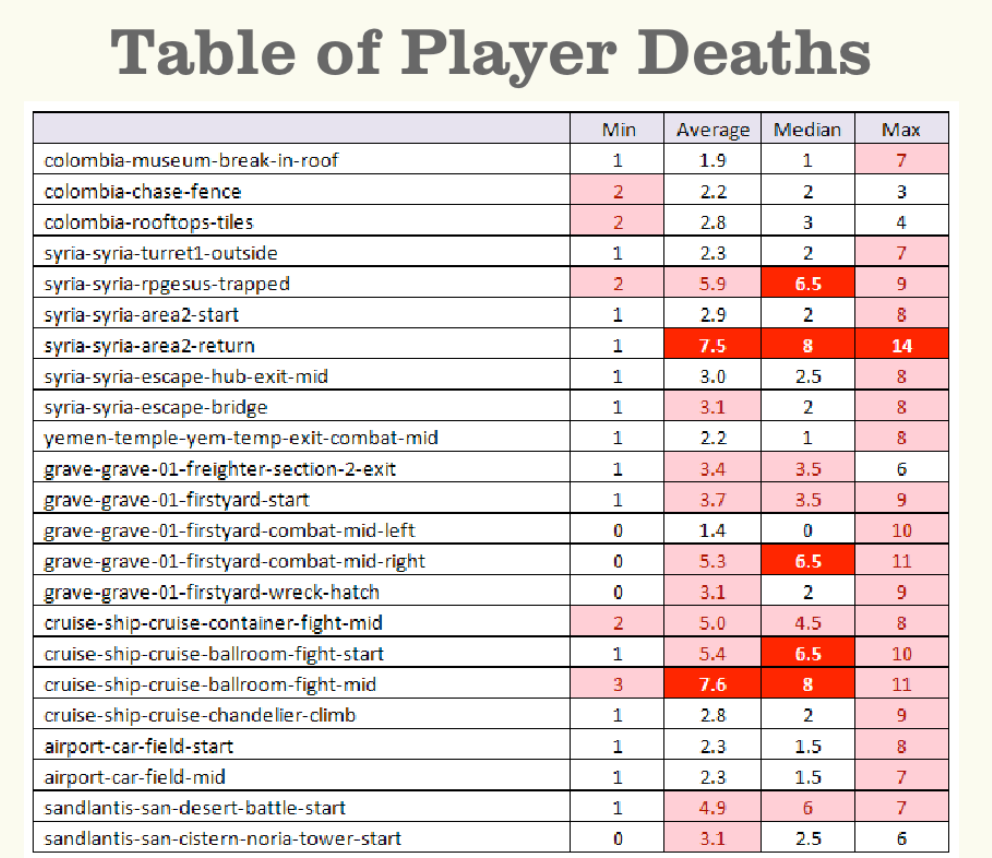
\includegraphics[scale=0.4]{PlayerDeathTable.png}
\end{center}

\begin{center}
\textit{Figure 1} \cite{GDCAttn:3}
\end{center}

\section{Postmortem Comparisons}

In Agile, the early research data gathered from playtesting can be used in sprint reviews and can mitigate the need for a large crunch at the end of development as bugs and design flaws can be spotted and fixed much sooner\cite{PMKOA:4}. More traditional methods may not catch these in this early stage. The longer that problems go unnoticed, the more work is put into problematic code, the more difficult and time consuming it becomes to fix later on \cite{GDCOTC:5}. This clearly advocates the idea that early, frequent playtesting is beneficial to development time and costs. \par
In more traditional methods like waterfall, testing is usually planned to be done at the end of a project \cite{ji2011comparing:6}. If playtesting is only used at the end of development for Quality Assurance, this can overwhelm a studio.  \cite{PMTrine:7}. Playtesting is about improving quality whereas QA is about making the game fully functional. Only allowing a few months to playtest a game before the final development stage is a risk to developers and investors. If the scope of the project has been underestimated then when it comes to the testing stage, a lack of funds or time to adequately playtest and do user research can easily become a reality\cite{PMZZ:8}. This can mean a lot more issues at launch particularly for large AAA games \cite{BrokenGames:9} or the game not being released at all. With an Agile approach, the continuous iteration can ensure that a shippable build is always available and with continuous testing and feedback, each iteration is more likely to be the best the game can be at that time. This significantly lowers the risk for investors, always knowing that launch is viable \cite{ghane2017quantitative:10}. This suggests that test-driven development in particular seems especially useful \cite{cunningham2005costs:11}. \par
Day one playtesting of a game by the developers through an early prototype can also be useful to focus the team \cite{Yampolsky:2016:LGD:2896958.2896965:12}. If you or other team members as developers are experiencing issues first-hand, it makes it difficult to ignore gameplay problems. This is very effective for small indie studio's who are making games with a smaller scope and constantly iterating over a basic build \cite{PMNS2:13}.


\section{How Early and How Often?}

Arguably, the most appropriate time to start playtesting is as soon as the developer has a question about the game \cite{GDCSharks:14}. This is likely to be very early on in the project and with Agile, and a flexible design document, user research about the game can be gathered in early iterations. With plan-driven development, this is a problem because the team has a large or rigid design document, and will be less likely to want to make changes before the end of development. \par
How often a game gets playtested depends on how often content or features are integrated and when special events are held. Playtesting throughout gives the developer a much better grip on the players experience, saves time and energy wasted on ineffective material, and gets the developer to focus on the nuances of a game. \cite{GDCAED:15}.


\section{The Community}

Early Access on Steam is a useful way of gaining user research data\cite{GamesEA:16}. 
Games that don't use Agile won't be able to go Early Access, as ideally this will happen well before the game is complete. This creates further funding for the game, and adds an early player base of testers who can provide feedback during development \cite{GDCOTC:5}. Methods such as waterfall would therefore be unable to benefit from EA. \par

There are risks however, such as if the initial release on EA isn't very appealing, perhaps because the gameplay mechanics are lacking. Normally this wouldn't be a huge problem, developers would be able to fix this in later iterations if playtesting was conducted within production. When the game has been released to the public in Early Access however, this can be an issue. The game will be judged by both players and press. People may forget about the game and therefore never see any of the improvements.

\section{Testing and Team Communication}

Testing early on in the development process can also be a boon to team communication as test-driven development promotes early communication between the different teams in a studio or company \cite{gallardo2009continuous:17}. Communication between the Product Owner, Testers, Designers and Programmers is paramount to ensuring a successful game is made \cite{mcdaniel2015communication:18}. 
Whereas if a studio elects to take a more plan-based approach or even an Agile approach with strict and inelastic procedures they may suffer \cite{cooke2012everything:19} \cite{davis2012agile:20}, communications may break down and team morale can be adversely affected \cite{cunningham2005costs:11}. This would hinder the development process overall and increase development times and costs.


\section{Conclusion}

It's clear that studios should use iteration \cite{o2015towards:21}, \cite{al2014towards:22} but should user research be part of that iterative process? Arguably, yes. Although much of the evidence presented in this paper is anecdotal and stems from research of various developers postmortems of their games, it is nonetheless a valuable insight into how user research is used in the development process of games today. Although using Agile doesn't rule out issues in larger companies, it does appear to limit them \cite{rico2009business:23}, \cite{batra2010balancing:24}. To summarise, the evidence clearly suggests that continuous playtesting and user research throughout the development process is very effective, especially in smaller teams. An argument can also be made that larger AAA companies should consider playtesting more often, even if they opt for a more waterfall approach to production.

\bibliographystyle{ieeetran}
\bibliography{references}

\end{document}




